%%%%%%%%%%%%%%%%%%%%%%%%%%%%%%%%%%%%%%%%%
% University Assignment Title Page 
% LaTeX Template
% Version 1.0 (27/12/12)
%
% This template has been downloaded from:
% http://www.LaTeXTemplates.com
%
% Original author:
% WikiBooks (http://en.wikibooks.org/wiki/LaTeX/Title_Creation)
%
% License:
% CC BY-NC-SA 3.0 (http://creativecommons.org/licenses/by-nc-sa/3.0/)
%
%%%%%%%%%%%%%%%%%%%%%%%%%%%%%%%%%%%%%%%%%
%\title{Title page with logo}
%----------------------------------------------------------------------------------------
%	PACKAGES AND OTHER DOCUMENT CONFIGURATIONS
%----------------------------------------------------------------------------------------

\documentclass[12pt]{article}
\usepackage[english]{babel}
\usepackage[utf8]{inputenc}
\usepackage{natbib}
\usepackage{amsmath}
\usepackage{color}
\usepackage[explicit]{titlesec}
\usepackage[hyphens,spaces,obeyspaces]{url}
\usepackage{graphicx}
\usepackage{caption}
\usepackage{subcaption}
\usepackage{grffile}
\usepackage{listings}

\lstset{language=python,keywordstyle={\bfseries \color{blue}}}


\begin{document}

\begin{titlepage}

\newcommand{\HRule}{\rule{\linewidth}{0.5mm}} % Defines a new command for the horizontal lines, change thickness here

\center % Center everything on the page
 
%----------------------------------------------------------------------------------------
%	HEADING SECTIONS
%----------------------------------------------------------------------------------------

\textsc{\LARGE University of St Andrews}\\[1.5cm] % Name of your university/college
\textsc{\Large Machine Learning}\\[0.5cm] % Major heading such as course name
\textsc{\large CS5014}\\[0.5cm] % Minor heading such as course title

%----------------------------------------------------------------------------------------
%	TITLE SECTION
%----------------------------------------------------------------------------------------

\HRule \\[0.4cm]
{ \huge \bfseries Classification}\\[0.4cm] % Title of your document
\HRule \\[1.5cm]
 
%----------------------------------------------------------------------------------------
%	AUTHOR SECTION
%----------------------------------------------------------------------------------------


\Large \emph{Author:}\\
 \textsc{150008022}\\[1cm] % Your name
 
%----------------------------------------------------------------------------------------
%	DATE SECTION
%----------------------------------------------------------------------------------------

{\large \today}\\[2cm] % Date, change the \today to a set date if you want to be precise

%----------------------------------------------------------------------------------------
%	LOGO SECTION
%---------------------------------------------------------------------------------------


\includegraphics[width = 4cm]{images/standrewslogo.png}
 
%----------------------------------------------------------------------------------------

\vfill % Fill the rest of the page with whitespace

\end{titlepage}

\subsection*{Goal}

The goal of this practical is to analyse a dataset in order to produce a classification model that can make predictions based on a set of inputs.

\tableofcontents

\pagebreak
\pagenumbering{arabic}
\setcounter{page}{1} 

\section{Loading Data}

To load the data, the paths to the relevant files are supplied as arguments to the \emph{\_\_main\_\_.py} script. The \emph{pandas} module was used to load the file contents into \emph{DataFrames}.

A test set was isolated from the original data using an 80\%-20\% split. Stratification was used to ensure that all classes were represented in the training data. 

% Merge data sets?

\section{Cleaning Data}

When originally loading the CSV files the parameter to raise an exception on missing or extra columns was included, and so it could be assumed that all rows had the same number of columns. The \lstinline{dtype=float} argument was also passed when loading the data to ensure that each column contained the expected numerical data. Any rows containing empty or \lstinline{NaN} values were dropped from the dataset.

\section{Data Visualisation and Analysis}

The input CSV was understood to have the structure shown in figure \ref{fig:structure} repeated once for each of the four channels.

\begin{figure}[!ht]
	\centering
	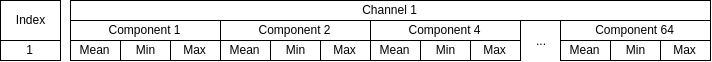
\includegraphics[width=\linewidth]{images/structure}
	\caption{The structure of each row of the CSV file which is repeated for each channel.}
	\label{fig:structure}
\end{figure}

% Samples to class ratio, all samples equally represented?

\subsection{Distributions}

\subsection{Relationships}

\section{Feature Selection}

The practical specification mentions that the data was collected in a slightly different way to the RadarCat paper \cite{radarcat}. 

Similiar features

\section{Model Selection and Training}
\subsection{Model 1}
\subsection{Model 2}
\section{Evaluation and Comparison}
\section{Discussion}

\bibliographystyle{unsrt}
\bibliography{mybib}

\end{document}
